%%%%%%%%%%%%%%%%%%%%%%%%%%%%%%%%%%%%%%%%%
% Jacobs Landscape Poster
% LaTeX Template
% Version 1.1 (14/06/14)
%
% Created by:
% Computational Physics and Biophysics Group, Jacobs University
% https://teamwork.jacobs-university.de:8443/confluence/display/CoPandBiG/LaTeX+Poster
% 
% Further modified by:
% Nathaniel Johnston (nathaniel@njohnston.ca)
%
% This template has been downloaded from:
% http://www.LaTeXTemplates.com
%
% License:
% CC BY-NC-SA 3.0 (http://creativecommons.org/licenses/by-nc-sa/3.0/)
%
%%%%%%%%%%%%%%%%%%%%%%%%%%%%%%%%%%%%%%%%%

%----------------------------------------------------------------------------------------
%	PACKAGES AND OTHER DOCUMENT CONFIGURATIONS
%----------------------------------------------------------------------------------------

\documentclass[final]{beamer}

\usepackage[scale=1.24]{beamerposter} % Use the beamerposter package for laying out the poster

\usetheme{confposter} % Use the confposter theme supplied with this template

\setbeamercolor{block title}{fg=nred,bg=white} % Colors of the block titles
\setbeamercolor{block body}{fg=black,bg=white} % Colors of the body of blocks
\setbeamercolor{block alerted title}{fg=white,bg=dred!70} % Colors of the highlighted block titles
\setbeamercolor{block alerted body}{fg=black,bg=dred!10} % Colors of the body of highlighted blocks
% Many more colors are available for use in beamerthemeconfposter.sty

%-----------------------------------------------------------
% Define the column widths and overall poster size
% To set effective sepwid, onecolwid and twocolwid values, first choose how many columns you want and how much separation you want between columns
% In this template, the separation width chosen is 0.024 of the paper width and a 4-column layout
% onecolwid should therefore be (1-(# of columns+1)*sepwid)/# of columns e.g. (1-(4+1)*0.024)/4 = 0.22
% Set twocolwid to be (2*onecolwid)+sepwid = 0.464
% Set threecolwid to be (3*onecolwid)+2*sepwid = 0.708

\newlength{\sepwid}
\newlength{\onecolwid}
\newlength{\twocolwid}
\newlength{\threecolwid}
\setlength{\paperwidth}{48in} % A0 width: 46.8in
\setlength{\paperheight}{36in} % A0 height: 33.1in
\setlength{\sepwid}{0.024\paperwidth} % Separation width (white space) between columns
\setlength{\onecolwid}{0.3\paperwidth} % Width of one column
\setlength{\twocolwid}{0.464\paperwidth} % Width of two columns
\setlength{\threecolwid}{0.708\paperwidth} % Width of three columns
\setlength{\topmargin}{-0.5in} % Reduce the top margin size
%-----------------------------------------------------------

\usepackage{graphicx}  % Required for including images

\usepackage{booktabs} % Top and bottom rules for tables

%----------------------------------------------------------------------------------------
%	TITLE SECTION 
%----------------------------------------------------------------------------------------

\title{Prediction of fund raising state of technology projects in Kickstarter using Machine Learning models} % Poster title


\author{Alonso Puente$^{1}$ , Marks Calderon$^{1}$} % Author(s)
\institute{$^{1}$ESAN University} % Institution(s)



%----------------------------------------------------------------------------------------

\begin{document}

\addtobeamertemplate{block end}{}{\vspace*{2ex}} % White space under blocks
\addtobeamertemplate{block alerted end}{}{\vspace*{2ex}} % White space under highlighted (alert) blocks

\setlength{\belowcaptionskip}{2ex} % White space under figures
\setlength\belowdisplayshortskip{2ex} % White space under equations

\begin{frame}[t] % The whole poster is enclosed in one beamer frame

\begin{columns}[t] % The whole poster consists of three major columns, the second of which is split into two columns twice - the [t] option aligns each column's content to the top

\begin{column}{\sepwid}\end{column} % Empty spacer column

\begin{column}{\onecolwid} % The first column



\begin{block}{Motivation}
Only \textbf{20\%} of Kickstarter technology projects were successful. It means this category has one of the lowest success rate.
	\begin{figure}
		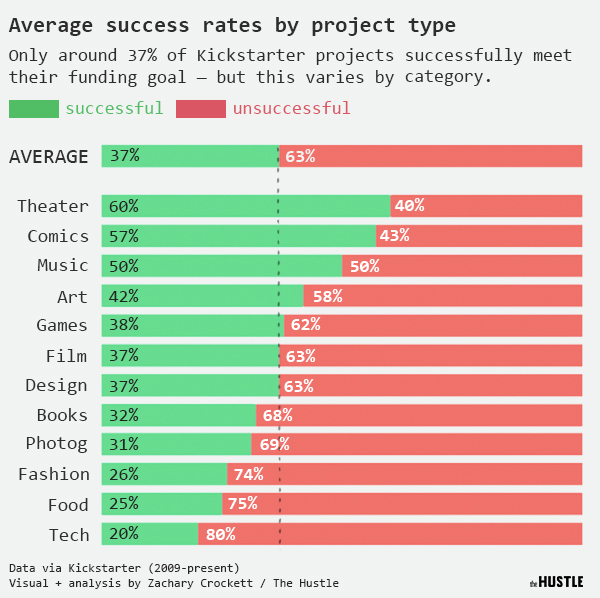
\includegraphics[width=0.5\linewidth]{kickstarter_success_rate_2009_2019.jpg}
		\caption{Kickstarter success rate, from 2009 to 2019}
	\end{figure}

In addition to this, previous researches were just focused on metadata variables, such as funding goal, number of backers, pledges, campaign duration, etc.
%------------------------------------------------

\end{block}

\begin{block}{Dataset and Features}
	We scraped \textbf{27,035} technology projects from Kickstarter, between 2009 and 2019. Those projects contained metadata (backers, goal, pledge and duration), visual content (project image) and textual content (project description).
	\begin{figure}
		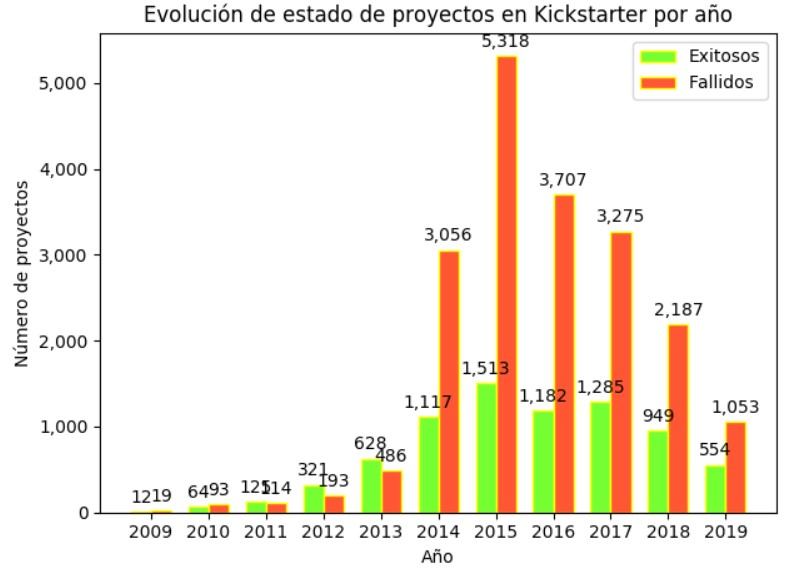
\includegraphics[width=0.75\linewidth]{scraped_projects.jpg}
		\caption{Success rate from Kickstarter's technology scraped projects.}
	\end{figure}
	
\end{block}

%----------------------------------------------------------------------------------------

\end{column} % End of the first column

\begin{column}{\sepwid}\end{column} % Empty spacer column



\begin{column}{\onecolwid} % The first column within column 2 (column 2.1)
	\begin{block}{Methods}
	Metadata start datasets were downloaded from WebRobots.io. Once the files were decompressed, they were pre-processed through \textbf{Alteryx Designer} software to build final datasets.
		
		\begin{figure}
			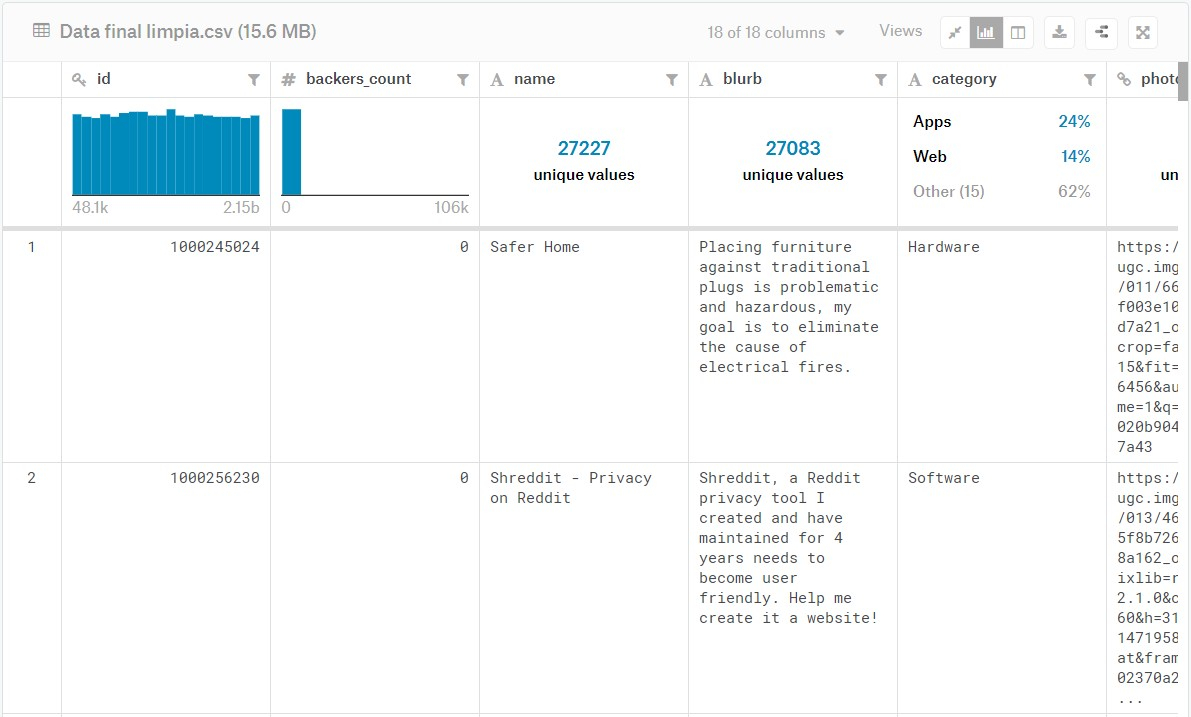
\includegraphics[width=0.8\linewidth]{metadata.jpg}
			\caption{Metadata variables scraped from Kickstarter}
		\end{figure}
	With projects URLs, project images and descriptions were scraped using Python libraries such as \textbf{Beautiful Soup} and \textbf{tqdm}.
	
	A framework based on the assembly of three predictive models for each part of the project was built:
		
		\begin{itemize}
			\item An \textbf{SVM} model for Metadata.
			\item A \textbf{Convolutional Neural Network (CNN)} for visual content.
			\item Two \textbf{SVM} models, the first one with \textbf{TF-IDF} and the second one with \textbf{BoW}.
		\end{itemize}
		
		\begin{figure}
			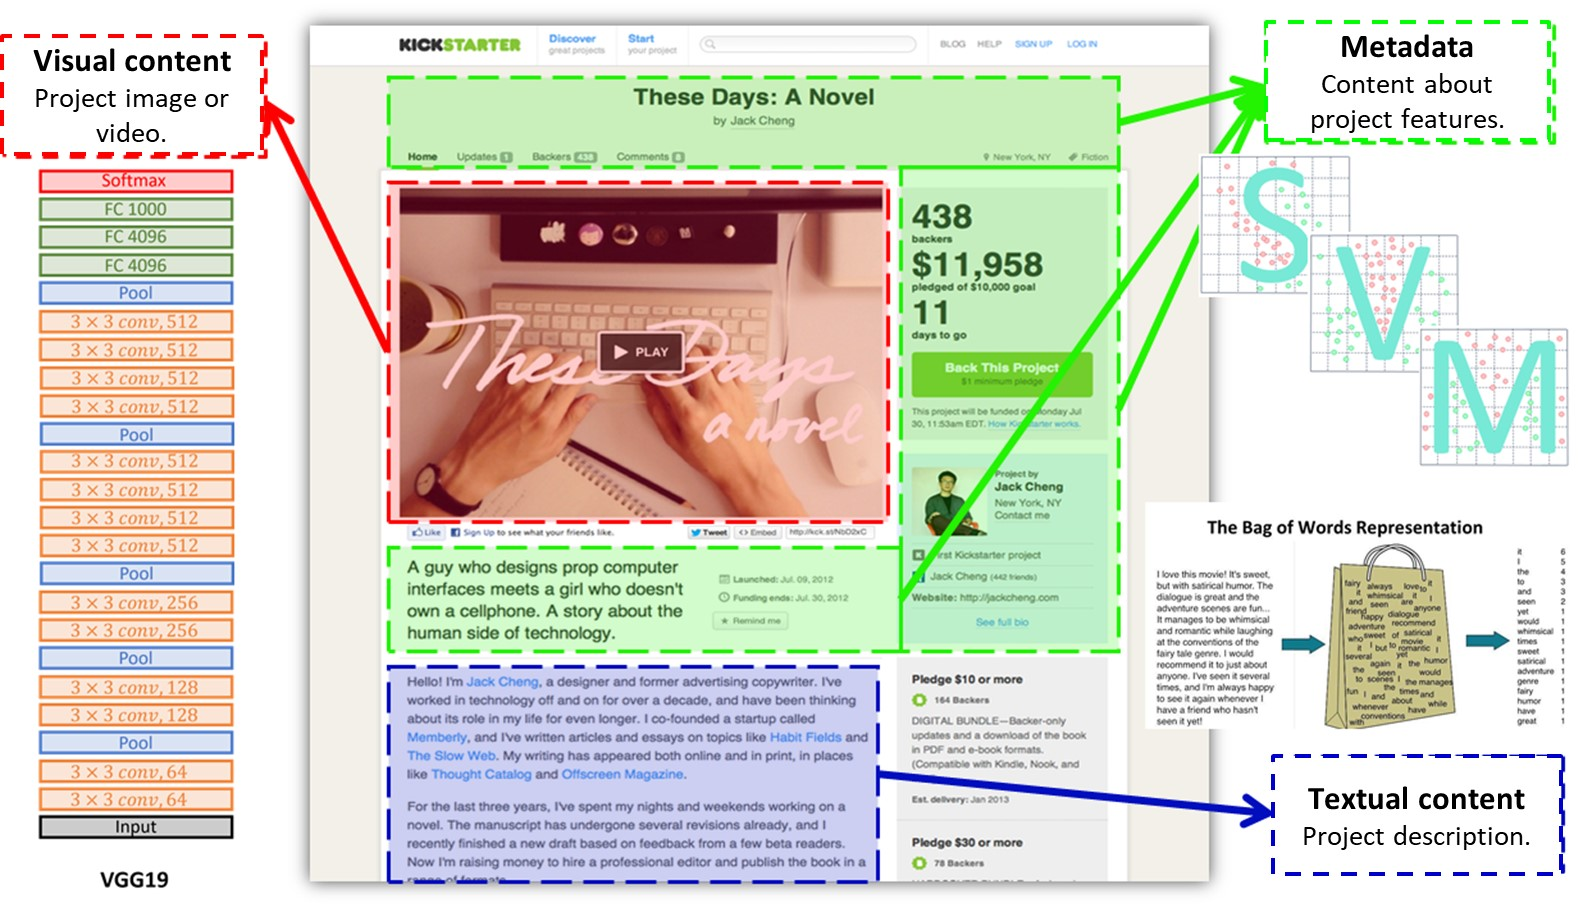
\includegraphics[width=0.95\linewidth]{prototipo.jpg}
			\caption{Proposed framework.}
		\end{figure}
		
	\end{block}


%----------------------------------------------------------------------------------------

\end{column} % End of column 2.1






\begin{column}{\sepwid}\end{column} % Empty spacer column

\begin{column}{\onecolwid} % The third column
	\begin{block}{Results and Discussion}
		
		According to selected evaluation metrics, each model obtained the following results after training stage:
		
		\begin{figure}
			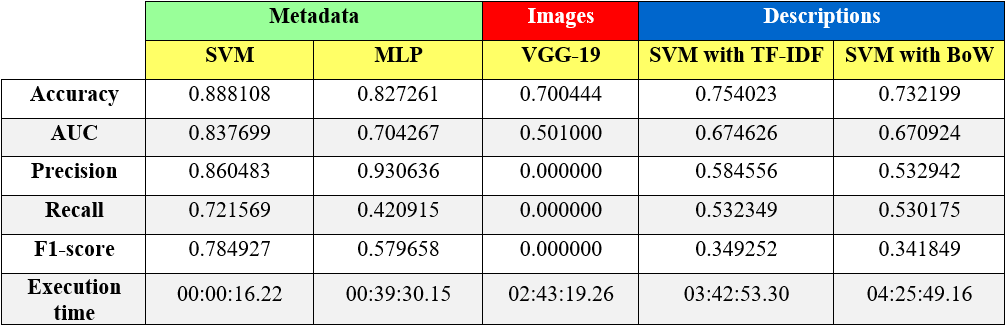
\includegraphics[width=0.8\linewidth]{resultados.png}
			\caption{Data training results.}
		\end{figure}
		
		Then, a demo was built in order to test metadata, images and description examples as inputs.
		
		\begin{figure}
			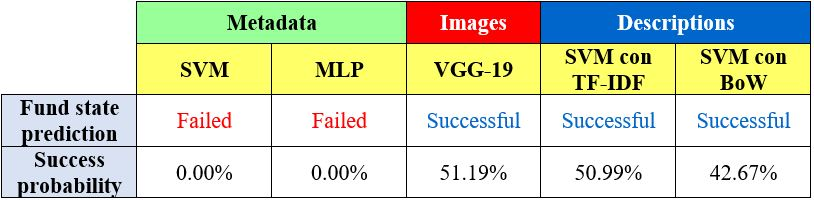
\includegraphics[width=0.8\linewidth]{demo.jpg}
			\caption{Demo results.}
		\end{figure}
		
	\end{block}
	\begin{block}{Conclusion and Discussion}
		
		After analyzing the models proposed for each part of the project, it was concluded that only the models for metadata and descriptions are acceptable to be used since the image model does not help to predict correctly due to falling into overfitting.
	\end{block}
	
	
	%----------------------------------------------------------------------------------------
	%	REFERENCES
	%----------------------------------------------------------------------------------------
	
	\begin{block}{References}
		
		\nocite{*} % Insert publications even if they are not cited in the poster
		\small{\bibliographystyle{unsrt}
			\bibliography{sample}\vspace{0.75in}}
		
	\end{block}


%----------------------------------------------------------------------------------------

\end{column} % End of the third column

\end{columns} % End of all the columns in the poster

\end{frame} % End of the enclosing frame

\end{document}
